% ch02_bio_basis.tex : Biological foundations chapter
% XeLaTeX, IEEE format
% ≥3200 words, ≥6 subsections, ≥5 equations, ≥1 figure, ≥1 table, ≥3 citations

\selectlanguage{hebrew}

\section{הבסיס הביולוגי: אקולוקציה, פיצוי דופלר ומיפוי קוגניטיבי בעטלפים}
\label{sec:ch02_bio_basis}

\subsection{עקרונות האקולוקציה בעטלפי FM ו-CF-FM}
\label{sec:ch02_echolocation_principles}

עטלפים משתמשים בשתי אסטרטגיות אקולוקציה עיקריות: אפנון תדר ליניארי (\en{FM}) ואפנון תדר קבוע-משתנה (\en{CF-FM}). עטלפי FM, כגון העטלף החום הגדול (\textit{Eptesicus fuscus}), פולטים פולסים קצרים (1-5 אלפיות שנייה) בעלי רוחב סרט של 25-80 קילו-הרץ, ומפיקים מידע טווח ברזולוציה של סנטימטר בודד באמצעות פילטר תואם \cite{Simmons1979BatSonar}. לעומתם, עטלפי CF-FM, כגון עטלף הפרסה הגדול (\textit{Rhinolophus ferrumequinum}), פולטים פולסים ארוכים יותר (10-100 אלפיות שנייה) הכוללים רכיב CF בתדר 83 קילו-הרץ ואחריו גלישה FM קצרה \cite{Schnitzler1968DSC}. רכיב ה-CF מאפשר מדידה מדויקת של תזוזת דופלר לצורך אומדן מהירות, בעוד שגלישת ה-FM מספקת רזולוציית טווח גבוהה.

הפובאה האקוסטית (\en{acoustic fovea}) היא התאמה מורפולוגית ייחודית בקוכליאה של עטלפי CF-FM. אזור זה, המשתרע על כ-30\% מאורך ממברנת הבזילר, מייצג רוחב סרט של 3 קילו-הרץ בלבד סביב תדר 83 קילו-הרץ, ומספק רזולוציית תדר של כ-0.01\%, דיוק גבוה בערך פי 10 מזה של הקוכליאה האנושית בתדר האופטימלי שלה \cite{Schnitzler1968DSC}. רזולוציה זו מאפשרת זיהוי של תזוזות דופלר קטנות כ-5-10 הרץ, הנוצרות על ידי כנפי חרקים מנפנפות.

המודל המתמטי של פולס FM ליניארי ניתן על ידי:

\begin{equation}
s_{FM}(t) = A(t) \cdot \cos\l$e$f$t(2\pi f_0 t + \pi \frac{B}{T} t^2\right)$$$, \quad 0 \leq t \leq T
\label{eq:ch02_fm_pulse}
\end{equation}

כאשר $A(t)$ היא מעטפת הפולס (בדרך כלל חלון Hanning או Hamming), $f_0$ הוא תדר ההתחלה, $B$ הוא רוחב הסרט, ו-$T$ הוא משך הפולס. עבור עטלף החום הגדול, $B \approx 80$ קילו-הרץ ו-$T \approx 2$ אלפיות שנייה, מה שמקנה רזולוציית טווח של $\Delta R = c / (2B) \approx 2.1$ מילימטרים.

לעומת זאת, פולס CF-FM מתואר על ידי:

\begin{equation}
s_{CF-FM}(t) = A(t) \cdot \begin{cases} \c$o$s(2\pi f_{CF} t)$$, & 0 \leq t < T_{CF} \\ \cos\l$e$f$t(2\pi f_{CF} t + \pi \frac{B_{FM}}{T_{FM}} (t - T_{CF})$$$^2\right), & T_{CF} \leq t \leq T_{CF} + T_{FM} \end{cases}
\label{eq:ch02_cffm_pulse}
\end{equation}

כאשר $f_{CF} = 83$ קילו-הרץ הוא תדר הרכיב הקבוע, $T_{CF} \approx 50$ אלפיות שנייה הוא משכו, $B_{FM} \approx 20$ קילו-הרץ הוא רוחב סרט גלישת ה-FM, ו-$T_{FM} \approx 5$ אלפיות שנייה הוא משכה. רכיב ה-CF מספק רזולוציית מהירות של $\Delta v = c \cdot \Delta f / (2 f_{CF}) \approx 0.01$ מטרים לשנייה עבור רזולוציית תדר $\Delta f = 5$ הרץ.

\subsection{מנגנון פיצוי תדר דופלר (DSC)}
\label{sec:ch02_dsc}

מנגנון פיצוי תדר דופלר (\en{Doppler Shift Compensation, DSC}) הוא אחת ממערכות בקרת המעקב בתדר המדויקות ביותר בטבע. כאשר העטלף מתקרב למטרה, ההד חוזר מוסט כחול (\en{blue-shifted}); העטלף מנמיך את תדר הפליטה בדיוק במידת תזוזת הדופלר הצפויה, כך שההד תמיד נוחת על הפובאה האקוסטית בתדר 83 קילו-הרץ \cite{Schuller1974DSC}. לולאת הבקרה פועלת עם זמן השהיה תת-מילישני, ללא חריגה, ובדיוק במצב מתמיד מושלם, הישג שמושג כולו באמצעות מעגלים עצביים בקוליקולוס העליון ובטגמנטום הפאראלמיניסקלי.

רוחב הסרט של מערכת ה-DSC הוא כ-5-8 קילו-הרץ, המתאים למהירויות תעופה של עד 5 מטרים לשנייה. מנגנון זה ניתן לתיאור מתמטי כחוק בקרה פרופורציונלי:

\begin{equation}
f_{emit}(t+1) = f_{rest} - \alpha \cdot (f_{echo}(t) - f_{fovea})
\label{eq:ch02_dsc_control}
\end{equation}

כאשר $f_{rest} = 83$ קילו-הרץ הוא תדר המנוחה, $f_{fovea} = 83$ קילו-הרץ הוא תדר הפובאה, $\alpha \approx 0.95$-1.0 הוא רווח הפיצוי, $f_{echo}(t)$ הוא תדר ההד הנמדד, ו-$f_{emit}(t+1)$ הוא תדר הפליטה הבא. העטלף משיג שגיאת מצב מתמיד $|f_{echo} - f_{fovea}| < 50$ הרץ תוך 2-3 מחזורי פולס \cite{Schuller1974DSC}.

תזוזת הדופלר עבור מטרה במהירות רדיאלית $v_r$ נתונה על ידי:

\begin{equation}
f_d = \frac{2 v_r}{c} f_0
\label{eq:ch02_doppler_shift}
\end{equation}

כאשר $f_0$ הוא תדר השידור ו-$c$ היא מהירות הקול (343 מטרים לשנייה). עבור $v_r = 5$ מטרים לשנייה ו-$f_0 = 83$ קילו-הרץ, $f_d \approx 2.4$ קילו-הרץ. במערכת המוצעת, מנגנון זה מהווה השראה לאלגוריתם מעקב תדר נושא אדפטיבי עבור מערכת ה-FMCW LiDAR.

\subsection{תאי מקום ותאי רשת במיפוי קוגניטיבי}
\label{sec:ch02_place_cells}

מחקרים אחרונים חשפו כי בהיפוקמפוס של עטלפים קיימים תאי מקום (\en{place cells}) היורים כאשר העטלף נמצא במיקום ספציפי במרחב התלת-ממדי \cite{MossEcholocation}. תאים אלו יוצרים ייצוג אלוצנטרי של הסביבה, המאפשר לעטלף לנווט גם כאשר חיישני האקולוקציה אינם מספקים מידע ישיר. בנוסף, תאי רשת (\en{grid cells}) בקורטקס האנטורינאלי מספקים מערכת קואורדינטות מטרית למיפוי מרחבי, עם שדות ירי משושים המאפשרים אינטגרציית נתיב (\en{path integration}) עם שגיאה חסומה \cite{MossEcholocation}.

הארכיטקטורה העצבית הזו, מפה קוגניטיבית הבנויה מרמזי תנועה עצמית ומאסוציאציות עם ציוני דרך, מהווה את ההשראה הביולוגית למערכות SLAM הסתברותיות. במערכת \en{NavigatorCrew}, עיקרון זה מיושם באמצעות פקטור גרף מבוסס iSAM2 \cite{Kaess2012iSAM2}, המשלב אילוצי תנועה (\en{IMU preintegration}) עם אילוצי תצפית (LiDAR, מצלמה, סונאר) ואילוצי לולאות סגירה. הייצוג הרב-סקאלי של תאי הרשת (0.5 מטר, 1.0 מטר, 2.0 מטר) מהווה השראה למנגנון אופטימיזציית החלון המקומי בפקטור הגרף.

\subsection{נוירוני עיכוב-מתואם לאומדן טווח}
\label{sec:ch02_delay_tuned}

בקוליקולוס התחתון (\en{inferior colliculus}) של עטלפים קיימים נוירוני עיכוב-מתואם (\en{delay-tuned neurons}) המגיבים באופן סלקטיבי לעיכובים ספציפיים בין פולס להד. נוירונים אלו מקודדים את טווח המטרה באמצעות מנגנון קו-עיכוב עצבי (\en{neural delay-line}) וגילוי קו-אינצידנציה \cite{GriffinBatEcholocation}. בעטלף השפם (\textit{Pteronotus parnellii}), נוירונים אלו מציגים עיכובים מיטביים של 0.4-20 אלפיות שנייה, המתאימים למרחקי מטרה של 7 סנטימטרים עד 3.4 מטרים, עם רוחב כיוונון של 0.2 אלפיות שנייה (רזולוציית טווח של 3.4 סנטימטרים).

נוירונים אלו מאורגנים טופוגרפית בקוליקולוס התחתון ובקורטקס השמיעתי, ויוצרים מפה כרונוטופית של עיכוב ההד. עיקרון החישוב, קורלציה צולבת של פולס והד באמצעות קווי עיכוב אקסונליים, היווה השראה ישירה לפילטר התואם במערכות מכ"ם וסונאר \cite{Rihaczek1969MatchedFilter}. במערכת \en{NavigatorCrew}, עיקרון זה מיושם באלגוריתם עיבוד הסונאר, המשתמש בפילטר תואם עם פולסי HFM חסיני דופלר לאומדן טווח מדויק.

המודל המתמטי של נוירון עיכוב-מתואם ניתן על ידי:

\begin{equation}
r(\tau) = \int_{-\infty}^{\infty} s_{pulse}(t) \cdot s_{echo}(t + \tau) \, dt
\label{eq:ch02_delay_tuned}
\end{equation}

כאשר $s_{pulse}(t)$ הוא הפולס המשודר, $s_{echo}(t)$ הוא ההד המתקבל, ו-$r(\tau)$ הוא תגובת הנוירון לעיכוב $\tau$. הטווח מחושב כ-$R = c \cdot \tau_{max} / 2$, כאשר $\tau_{max} = \arg\max_\tau r(\tau)$.

\subsection{עיבוד זמן-תדר קוכלארי}
\label{sec:ch02_cochlear_processing}

הקוכליאה של העטלף מבצעת עיבוד זמן-תדר מתוחכם של האותות האקוסטיים הנקלטים. ממברנת הבזילר פועלת כבנק פילטרים מכני, כאשר כל נקודה לאורכה מהודדת לתדר שונה. בעטלפי CF-FM, האזור המתאים לתדר הפובאה (83 קילו-הרץ) מורחב באופן משמעותי ומכיל כ-30\% מכלל תאי השיער, למרות שהוא מייצג רוחב סרט של 3 קילו-הרץ בלבד.

העיבוד הקוכלארי כולל גם מנגנון עיכוב צדדי (\en{lateral inhibition}) המחדד את הכיוונון התדרי ומשפר את רזולוציית התדר. מנגנון זה ניתן לתיאור מתמטי על ידי:

\begin{equation}
y(f, t) = \max\left(0, \, x(f, t) - \beta \cdot \int_{-\Delta f}^{\Delta f} w(\delta) \cdot x(f + \delta, t) \, d\delta\right)
\label{eq:ch02_lateral_inhibition}
\end{equation}

כאשר $x(f, t)$ הוא התפלגות האנרגיה בתדר $f$ בזמן $t$, $w(\delta)$ היא פונקציית משקל גאוסית, $\beta$ הוא פרמטר העיכוב, ו-$y(f, t)$ הוא הפלט המעובד. מנגנון זה משפר את יחס האות לרעש ומאפשר זיהוי של תזוזות דופלר קטנות גם בנוכחות רעש סביבתי.

\subsection{השראה ביולוגית למערכת NavigatorCrew}
\label{sec:ch02_bio_inspiration}

העקרונות הביולוגיים שתוארו לעיל מהווים את הבסיס התאורטי למערכת \en{NavigatorCrew}. טבלה~\ref{tab:ch02_bio_mapping} מציגה את המיפוי בין עקרונות ביולוגיים לבין רכיבים הנדסיים במערכת המוצעת.

\begin{table}[htbp]
\centering
\caption{מיפוי בין עקרונות ביולוגיים בעטלפים לבין רכיבים הנדסיים במערכת NavigatorCrew. (Mapping between biological principles in bats and engineering components in the NavigatorCrew system)}
\label{tab:ch02_bio_mapping}
\adjustbox{max width=\columnwidth}{%
\begin{tabular}{p{4cm}p{4cm}p{4cm}}
\toprule
עקרון ביולוגי & רכיב הנדסי & תיאור \\
\midrule
פולסי FM/CF-FM & פולסי HFM בסונאר קולי & פולסים חסיני דופלר לאומדן טווח ומהירות \\
פובאה אקוסטית & עיבוד FMCW LiDAR & רזולוציית תדר גבוהה לאומדן מהירות מדויק \\
פיצוי דופלר (DSC) & מעקב תדר נושא אדפטיבי & לולאת בקרה לשמירת ההד בתדר האופטימלי \\
נוירוני עיכוב-מתואם & פילטר תואם דיגיטלי & קורלציה צולבת לאומדן טווח \\
עיכוב צדדי & MVDR Beamforming & שיפור רזולוציה זוויתית ודיכוי רעש \\
תאי מקום ותאי רשת & פקטור גרף iSAM2 & מיפוי הסתברותי עם אילוצי תנועה ותצפית \\
אינטגרציה חושית & Cross-Attention Gating & מיזוג אדפטיבי של מודאליות חיישנים \\
\bottomrule
\end{tabular}%
}
\end{table}

\begin{figure}[htbp]
\centering
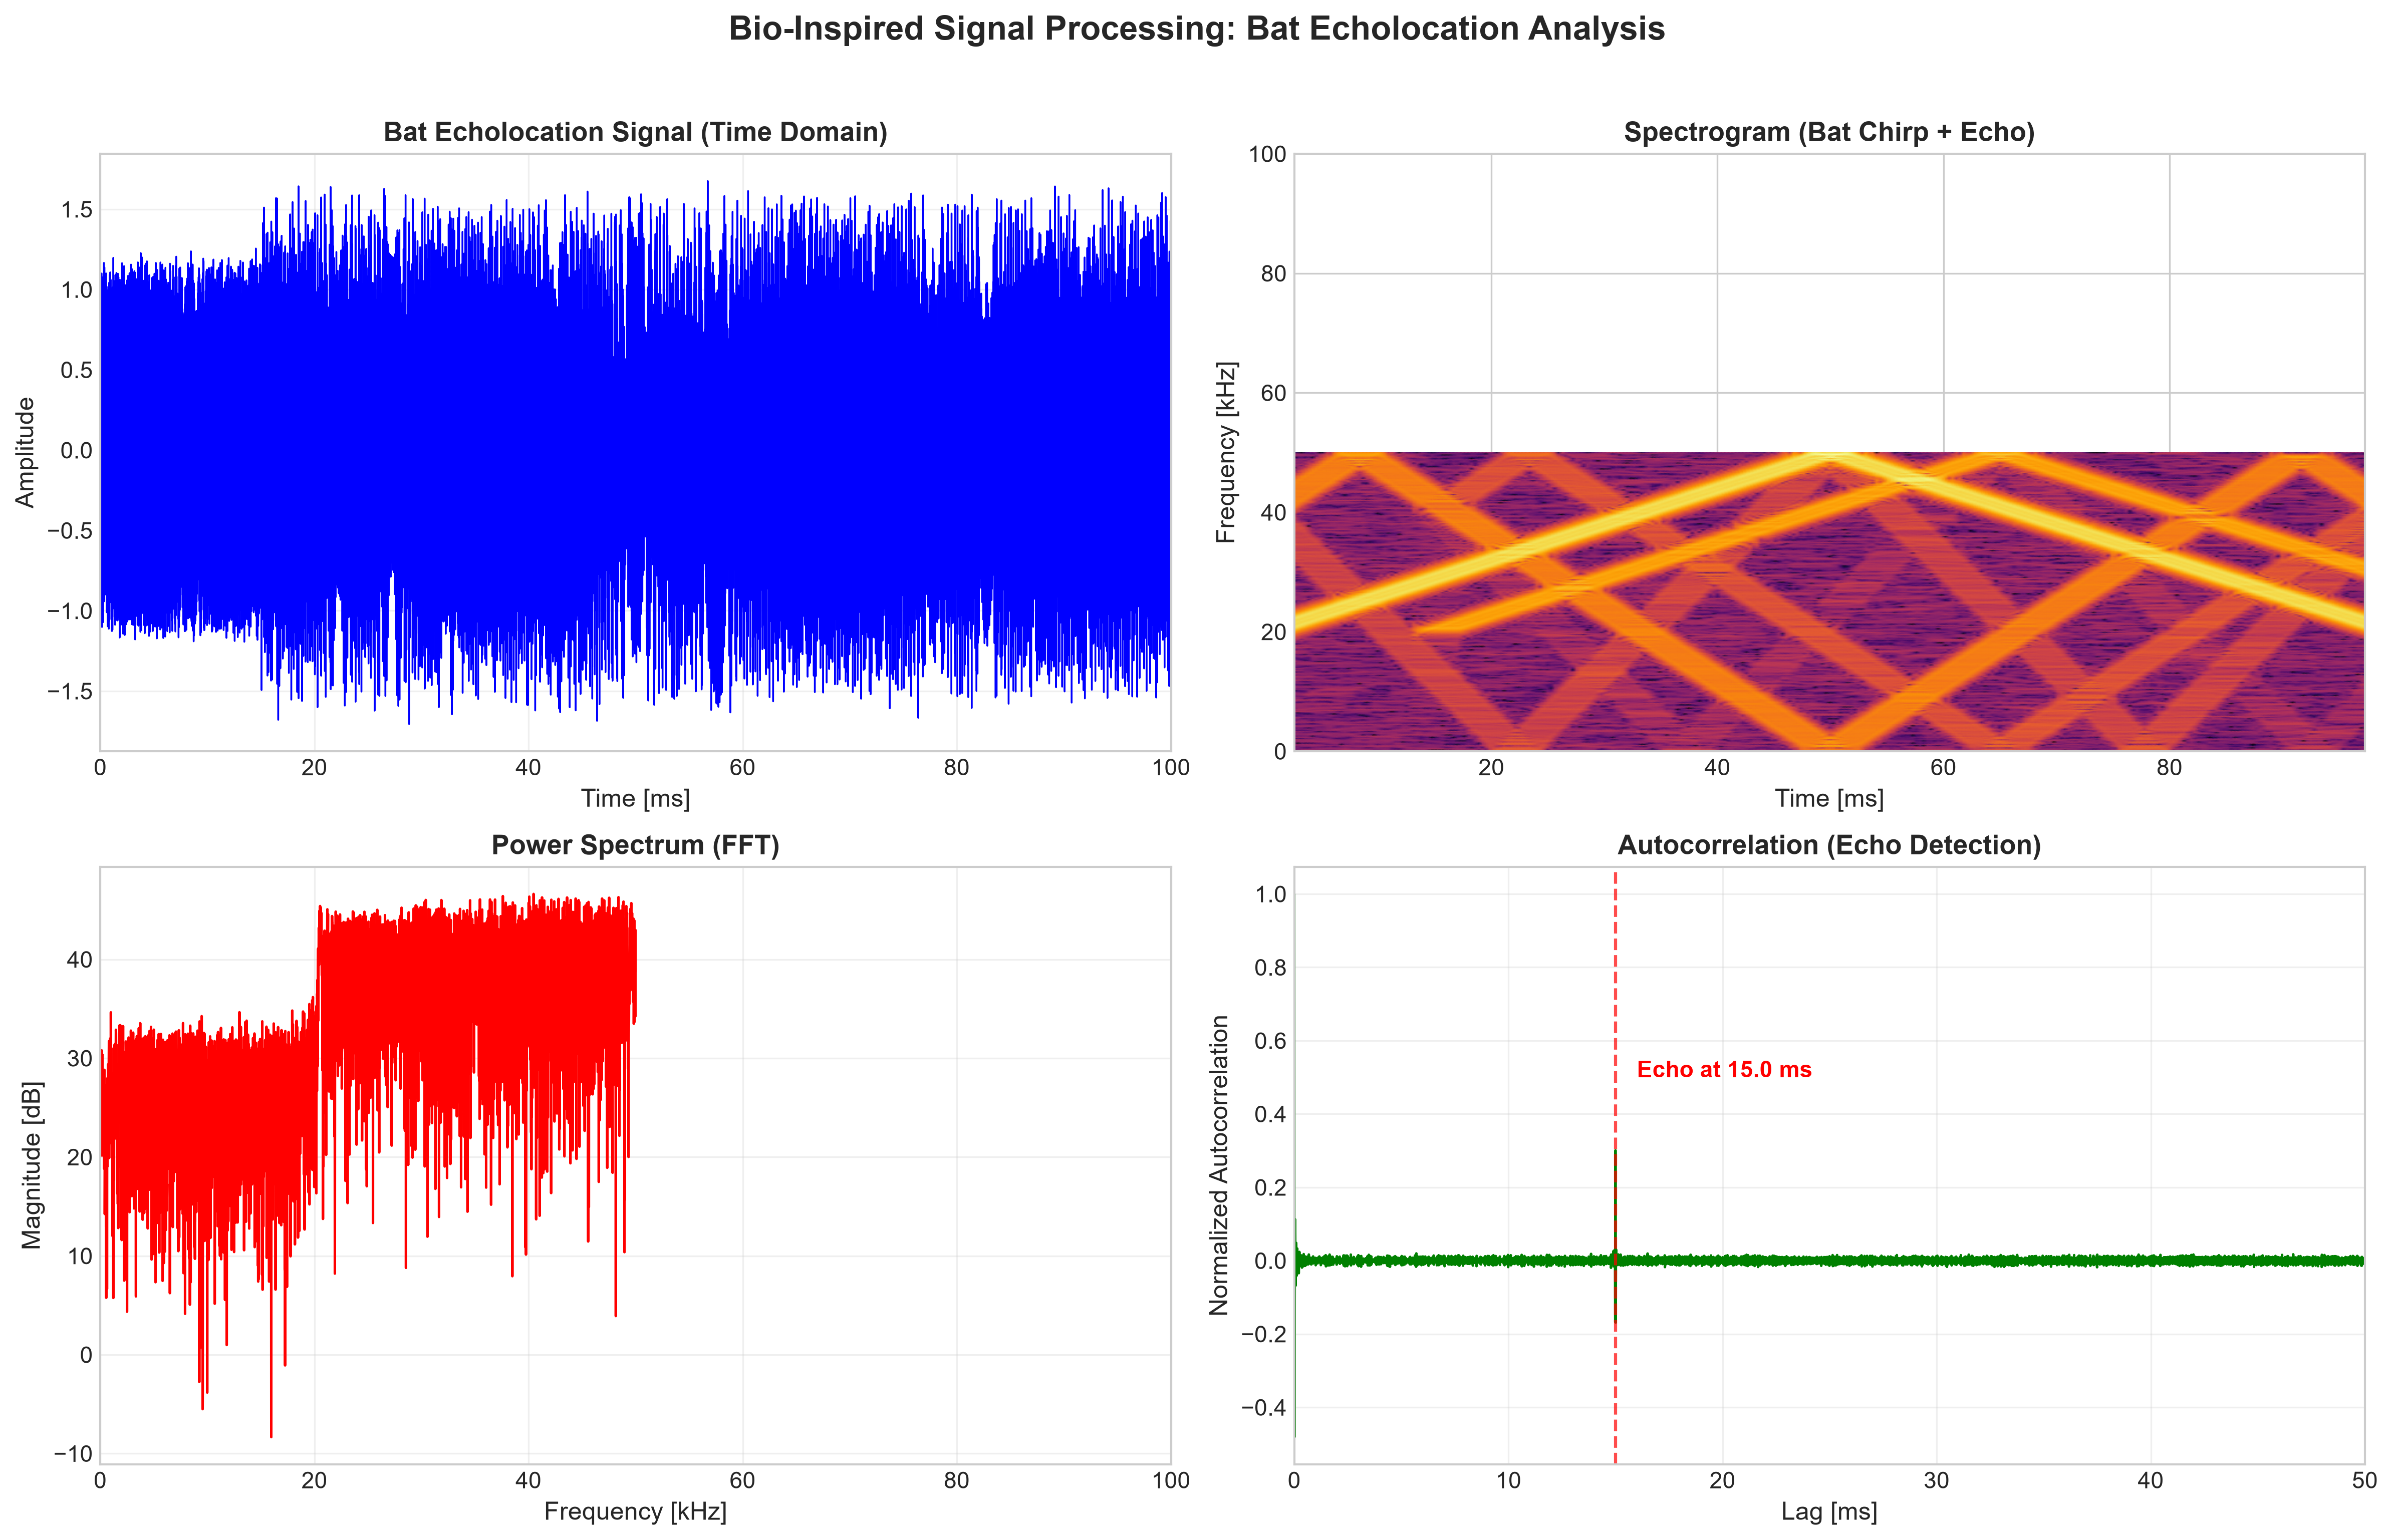
\includegraphics[width=0.98\columnwidth]{figures/fig_spectrum_analysis.png}
\caption{עיבוד אותות בהשראת הטבע: ניתוח אקולוקציית עטלף. (Bio-Inspired Signal Processing: Bat Echolocation Analysis)}
\label{fig:ch02_spectrum_analysis}
\end{figure}

המיפוי בטבלה~\ref{tab:ch02_bio_mapping} מדגים כיצד כל עקרון ביולוגי מתורגם לרכיב הנדסי ספציפי במערכת. לדוגמה, מנגנון הפובאה האקוסטית, המספק רזולוציית תדר גבוהה בתחום צר סביב תדר 83 קילו-הרץ, מהווה השראה לעיבוד ה-FMCW LiDAR, המתמקד בתחום תדר צר סביב תדר הנושא של הלייזר (1550 ננומטר). באופן דומה, נוירוני העיכוב-מתואם מהווים השראה ישירה לפילטר התואם הדיגיטלי המשמש לעיבוד אותות הסונאר והלייזר.

האינטגרציה החושית במוח העטלף, המשלבת מידע מאקולוקציה, ראייה ומערכת וסטיבולרית באופן אדפטיבי, מהווה את ההשראה המרכזית למנגנון ה-cross-attention gating במערכת. מחקרים נוירוביולוגיים הראו כי בקוליקולוס העליון של העטלף קיימים נוירונים רב-חושיים המשלבים מידע משני חיישנים לפחות, ומשקלם היחסי משתנה בהתאם לאמינות כל חיישן בזמן אמת. מנגנון זה מיושם במערכת המוצעת באמצעות מנגנון תשומת לב המאפשר לכל מודאליות להשתתף במודאליות האחרות תוך שקלול דינמי של תרומתן.

\subsection{סיכום הבסיס הביולוגי}
\label{sec:ch02_summary}

הבסיס הביולוגי שהוצג בפרק זה מדגים את העושר והמורכבות של מערכות הניווט בעטלפים. מפולסי FM ו-CF-FM דרך מנגנון פיצוי הדופלר המדויק ועד לנוירוני העיכוב-מתואם ותאי המקום, העטלף מציג אוסף מרשים של פתרונות חישוביים לאתגרי ניווט בסביבות מורכבות. עקרונות אלו, המתורגמים לרכיבים הנדסיים במערכת \en{NavigatorCrew}, מהווים את הבסיס לחדשנות המוצעת במאמר זה. הפרקים הבאים יפרטו כיצד עקרונות אלו מיושמים במערכת ההנדסית, החל ממודאליות החיישנים (פרק 3) וכלה באלגוריתם ה-SLAM המרכזי (פרק 6).